\section{Theorie}
\label{sec:Theorie}

%Quantenzahlen
\subsection{Gesamtwellenfunktion und Quantenzahlen}
Die Lösung des Wasserstoffproblems liefert die Wellenfunktion
\begin{equation*}
    \Psi_{n, l, m} (x, y, z) = R_{n, l}(r) \cdot Y_l^m (\vartheta, \varphi) \cdot \chi_{m_s}
\end{equation*}
, welche die Verteilung der Aufenthaltswahrscheinlichkeit eines Elektronens angibt.\\
Die Quantenzahl $n = 1, 2, 3 ...$ wird als Hauptquantenzahl bezeichnet, diese gibt die Elektronenschale bzw. das Energieniveau an zu dem der Zustand des Elektrons gehört.
Die Nebenquantenzahl $l = 0, 1, 2, ..., n-1 $ wird auch Drehimpulsquantenzahl genannt, da dieser nach \autoref{eqn:eigenwert_l} den Eigenwert vom Quadrat des Drehimpulsoperators angibt. 
Um die räumliche Orientierung des Drehimpulses anzugeben, wird die Magnetische Quantenzahl $m = \frac{L_z}{\hbar} = -l, - (l-1), ..., (l-1), l$ verwendet.
Die Spinquantenzahl $s = -\frac{1}{2} , \frac{1}{2}$ gibt den Spin an.
\\ \\
Der Bahndrehimpuls und der Elektronenspin stehen wie folgt mit den Quantenzahlen in Relation:
\begin{align}
    |\vec{l}| &= \sqrt{l(l+1)} \hbar \label{eqn:eigenwert_l} \\
    |\vec{s}| &= \sqrt{s(s+1)} \hbar \label{eqn:eigenwert_s}
\end{align}

%Normaler Zeeman
\subsection{Normaler Zeeman-Effekt}
\subsubsection{Allgemein}
Wird ein Atom in ein Magnetfeld $B$ gebracht, so spalten sich die $(2l + 1)$ entarteten Spektrallinien in $(2l + 1)$ äquidistante Energieniveaus auf (siehe Abb. \ref{fig:zeeman_aufspaltung}).
Die Aufspaltung der Spektrallinien, die durch das magnetischen Moment des Bahndrehimpuls $l$ \eqref{eqn:eigenwert_l} erzeugt wird, wird als normaler Zeeman-Effekt bezeichnet.
Das Bohr'sche Magneton
\begin{equation}
    \mu_B = \frac{e \cdot \hbar}{2 m_e}
    \label{eqn:magneton}
\end{equation}
gibt im Bohr'schen Atommodell den Betrag des magnetischen Moments eines Elektrons im Grundzustand an.
Hierbei steht $e$ für die Elementarladung, $\hbar$ für das reduzierte Plancksche Wirkungsquantum und $m_e$ für die Ruhemasse des Elektrons.

Der Abstand der Zeeman-Komponenten ist konstant und beträgt
\begin{equation*}
    \Delta E = E_{n,l,m} - E_{n,l,m-1} = \mu_B \cdot B \, .
\end{equation*}
\\
\begin{figure}
    \centering
    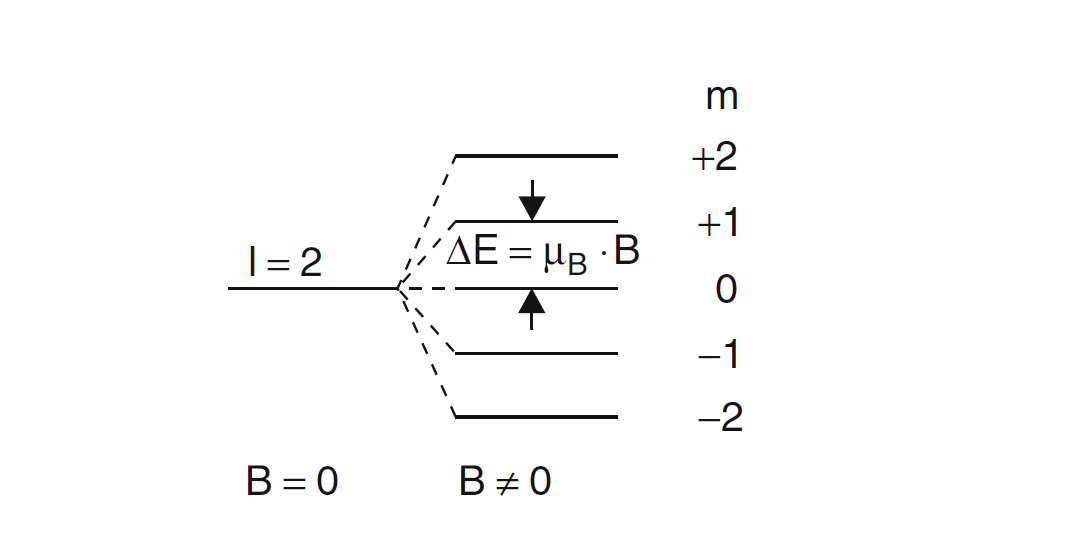
\includegraphics[width=0.8\textwidth]{content/data/zeeman_aufspaltung.png}
    \caption{Schematische Darstellung des Zeeman-Effekts. Die Spektrallinien spalten sich unter Einfluss eines Magnetfeldes auf.} %ref
    \label{fig:zeeman_aufspaltung}
\end{figure}

Das magnetische Bahnmoment des Elektrons bzw. das magnetische Moment des Drehimpulses
\begin{equation}
    \vec{\mu_l} = -\frac{\mu_B}{\hbar} \cdot \vec{l}
    \label{eqn:magn_moment_l}
\end{equation}
ergibt sich aus dem Bohrschen Magneton $\mu_B$ \eqref{eqn:magneton}, dem reduzierten plankschen Wirkungsquantum $\hbar$ und dem Einheitsvektor $\vec{l}$.
 
\subsubsection{Emission und Absorption von Licht}
Betrachtet man Emission und Absorption von Licht durch Atome in einem Magnetfeld mit $\vec{B} = B \cdot \vec{z}$ wird folgendes beobachtet:

\begin{itemize}
    \item fällt $\sigma^+$-polarisiertes Licht in $z$-Richtung auf ein Atom, so treten Übergänge mit $\Delta m = +1$ auf
    \item analog dazu treten bei $\sigma^-$-polarisiertem Licht Übergänge mit $\Delta m = -1$ auf
    \item bei der Emission von Photonen, werden dem entsprechend $\sigma^+ -$ und $\sigma^-$-Licht in Feldrichtung $\vec{z}$ beobachtet
    \item senkrecht zum Magnetfeld werden drei linear polarisierte Komponenten gemessen (2 senkrecht und eine parallel zu $\vec{z}$)
    \item die Spektrallinien werden bei einem Übergang zwischen zwei Zuständen in drei Zeeman-Komponenten aufgespalten: $\sigma^+$, $\sigma^-$, $\pi$ -Polarisation
\end{itemize}